% import packages
\documentclass[10pt]{beamer}
\usepackage[utf8]{inputenc}
\usepackage{graphicx}
\usepackage{hhline}
\usepackage{amsmath}
\usepackage{amssymb}
\usepackage{tikz}
\usepackage[justification=centering]{caption}
\usepackage[backend=bibtex,style=authoryear-comp,dashed=false,natbib=true]{biblatex}

% set beamer parameters
\setbeamerfont{footnote}{size=\Tiny}
\setbeamertemplate{navigation symbols}{}
\setbeamertemplate{page number in head/foot}{}
\setbeamertemplate{bibliography item}{}
\setbeamertemplate{caption}[numbered]
\setbeamercovered{transparent}
\setbeamerfont{institute}{size=\small}
\usetheme{Frankfurt}
\usecolortheme{whale}
\setbeamertemplate{footline}{% 
	\hfill% 
	\usebeamercolor[fg]{page number in head/foot}% 
	\usebeamerfont{page number in head/foot}% 
	\insertframenumber%
	%\,/\,\inserttotalframenumber
	\kern1.2em\vskip4.5pt% 
}

% set caption parameters
\DeclareCaptionFormat{myformat}{\fontsize{6}{6}\selectfont#1#2#3}
\captionsetup{format=myformat}
\captionsetup[figure]{labelfont={bf},name={Figure}}
\captionsetup[table]{labelfont={bf},name={Table}}

% set bibliography parameters
\renewcommand\refname{Bibliography}
\addbibresource{../bibtex.bib}
\setlength\bibitemsep{1.5\itemsep}
\let\oldcitep=\citep
\renewcommand\citep[1]{{\textcolor{blue}{\oldcitep{#1}}}}
\let\oldcitet=\citet
\renewcommand\citet[1]{{\textcolor{blue}{\oldcitet{#1}}}}

% miscellaneous settings
\settowidth{\leftmargini}{\usebeamertemplate{itemize item}}
\addtolength{\leftmargini}{\labelsep}
\renewcommand{\arraystretch}{1.3}
\graphicspath{{../visuals/}}

% set admin details
\title{SoPa++: Leveraging explainability from hybridized RNN, CNN and weighted finite-state neural architectures}
\author{Atreya Shankar, \texttt{shankar@uni-potsdam.de} \\ Cognitive Systems: Language, Learning, and Reasoning (M.Sc.)}
\institute{Thesis Progress Update \\ University of Potsdam, WiSe 20/21 \vspace{-5pt}}
\date{\today}

% start presentation
\begin{document}
\begin{frame}
  \maketitle
\end{frame}

\section{Introduction}

\subsection{}
\begin{frame}
  \frametitle{Recap}
  \begin{enumerate}
    \setbeamertemplate{enumerate items}[square] \setlength\itemsep{0.8em}
    \item Source code refactored to work with latest \texttt{PyTorch} and
    \texttt{CUDA} versions
    \item Facebook NLU multi-class intent detection data set from
    \citet{schuster-etal-2019-cross-lingual}
    \item Performance is important for explainability, because it does not make
    sense to explain a poorly performing model
    \item Focus would be to develop SoPa++ as a neural model which can be easily
    decomposed into a \textit{globally} explainable model
  \end{enumerate}
\end{frame}

\section{Background}

\subsection{}
\begin{frame}
  \frametitle{Semirings}
  \textbf{\citealt{kuich1986linear}:}\\
  A semiring is a set $\mathbb{K}$ along with two binary associative operations $\oplus$ (addition) and $\otimes$ (multiplication) and two identity elements: $\bar{0}$ for addition and $\bar{1}$ for multiplication. Semirings require that addition is commutative, multiplication distributes over addition, and that multiplication by $\bar{0}$ annihilates, i.e., $\bar{0} \otimes a = a \otimes \bar{0} = \bar{0}$\\
  \vspace{10pt}
  \begin{itemize}
    \item Generic semiring notation: $\langle \mathbb{K}, \oplus, \otimes,
    \bar{0}, \bar{1} \rangle$
    \item Max-sum semiring: $\langle \mathbb{R} \cup \{-\infty\}, \text{max}, +,
    -\infty, 0 \rangle$
    \item Max-product semiring: $\langle \mathbb{R} \cup \{-\infty\},
    \text{max}, \times, -\infty, 1 \rangle$
    \item Many semirings are possible, but we stick to \textit{max} based
    semirings
  \end{itemize}
\end{frame}

\subsection{}
\begin{frame}
  \frametitle{Weighted Finite-State Automata}
  \begin{equation}
    p(\pmb{x}) = \pmb{\pi} \otimes \Bigg( \bigotimes_{i=1}^n \pmb{T}(x_i) \Bigg) \otimes \pmb{\eta}
  \end{equation} 
  \begin{equation}
    s(\pmb{z}) = \bigoplus_{\pmb{x} \in \Pi(\pmb{z})} p(\pmb{x})
  \end{equation}
  \vspace{10pt}
  \begin{itemize}
    \item Path $\pmb{x} = \langle x_1, x_2, \dots, x_n \rangle$ derives some
    string $\pmb{z} = \langle z_1, z_2, \dots, z_m \rangle$
    \item $\Pi(\pmb{z})$ is the set of all possible paths that derive string
    $\pmb{z}$
    \item $\pmb{\pi}$, $\pmb{\eta}$ are start and end state vectors
    \item $\pmb{T}$ is a transition matrix defining transition scores between
    states
    \item $p(\pmb{x})$ refers to a score through a particular path
    \item $s(\pmb{z})$ refers to an aggregate score through all possible paths
    \item Utilize Viterbi algorithm with \textit{max} based semirings to compute
    $s(\pmb{z})$ \citep{viterbi1967error}
  \end{itemize}
\end{frame}

\section{SoPa++}
\subsection{}
\begin{frame}
  \frametitle{Finite transition types}
  \begin{figure}
    \captionsetup{justification=centering}
    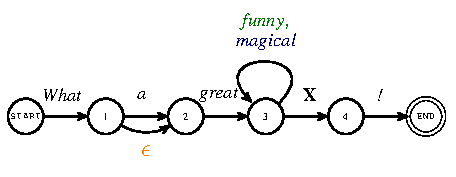
\includegraphics[width=10cm]{pdfs/borrowed/linear_fsa_special_transitions.pdf}
    \caption{Schematic for finite-state transitions; $\epsilon$ represents an
      epsilon-transition, ``funny'' and ``magical'' form self-loops and all
      other transitions are main transitions \citep{schwartz2018sopa}}
  \end{figure}
  \begin{itemize}
    \item Vanilla SoPa allowed 3 transitions types: main, epsilon and self-loops
    \item \textbf{SoPa++ uses only two transitions: namely main and wildcard
      transitions}
    \item Both consume one token and one state, which leads to pattern-string
    determinism and could make the \textit{explainability} step easier
  \end{itemize}
\end{frame}

\subsection{}
\begin{frame}
  \frametitle{SoPa++: Lower Model}
  \begin{figure}
    \captionsetup{justification=centering}
    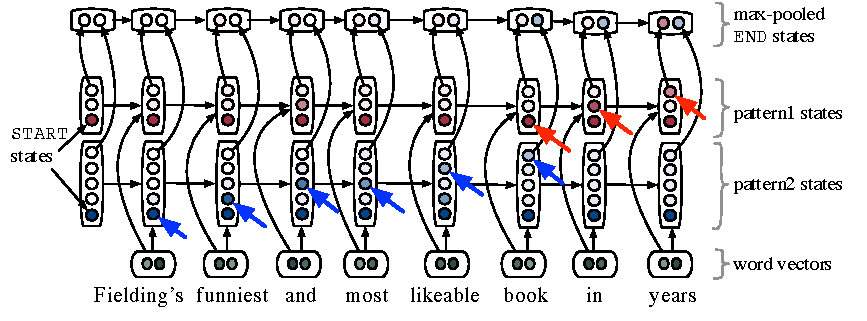
\includegraphics[width=11cm]{pdfs/borrowed/sopa_computational_graph.pdf}
    \caption{SoPa++ lower model schematic where pattern 1 is activated by the
      substring ``in years'' and pattern 2 is activated by the substring
      ``funniest and most likeable book'' \citep{schwartz2018sopa}}
  \end{figure}
  \begin{itemize}
    \setlength\itemsep{0.6em}
    \item Vanilla SoPa places a MLP on top of the max-pooled states to retrieve
    classification results
    \item This contributes to a lack of explainability since MLPs are generally
    not easily explainable
  \end{itemize}
\end{frame}

\subsection{}
\begin{frame}
  \frametitle{SoPa++: Upper Model}
  \begin{figure}
    \captionsetup{justification=centering}
    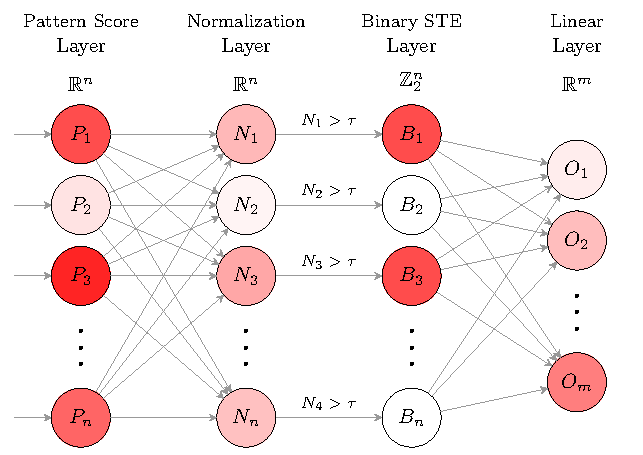
\includegraphics[width=10cm]{pdfs/generated/spp_upper_diagram/main.pdf}
    \caption{SoPa++ upper model schematic (combined lower-upper schematic
      under-construction); STE refers to a straight-through-estimator
      \citep{yin2019understanding}}
  \end{figure}
\end{frame}

\subsection{}
\begin{frame}
  \frametitle{SoPa++: Explainable Model}
  \begin{figure}
    \captionsetup{justification=centering}
    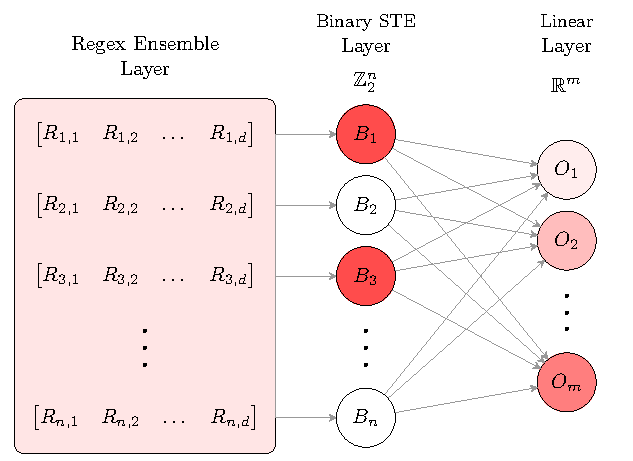
\includegraphics[width=9.5cm]{pdfs/generated/regex_diagram/main.pdf}
    \caption{SoPa++ explainable variant derived from antecedent neural model}
  \end{figure}
\end{frame}

\section{Results}
\subsection{}
\begin{frame}
  \frametitle{Training and Convergence}
  \begin{figure}
    \captionsetup{justification=centering}
    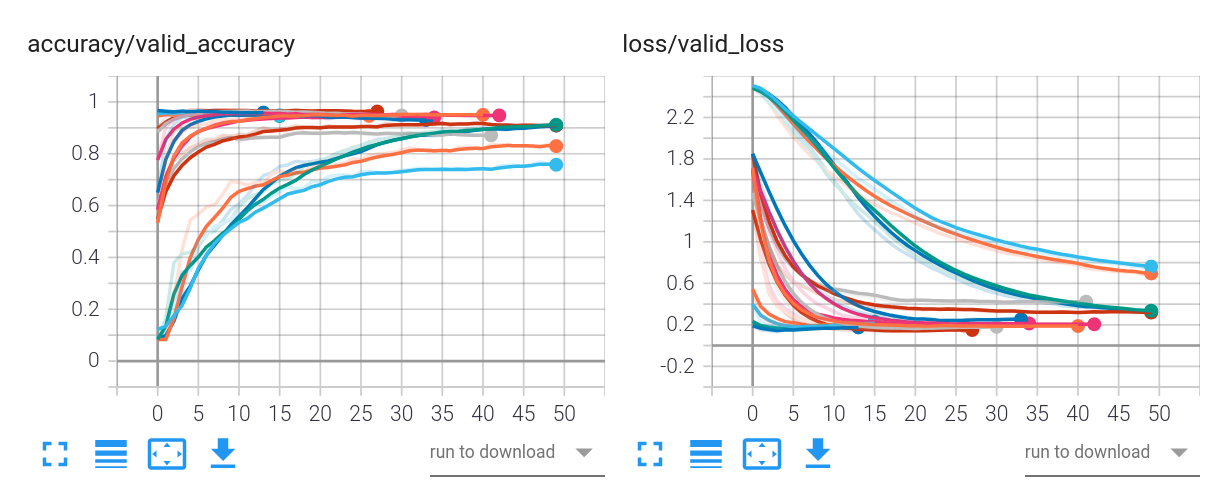
\includegraphics[width=10cm]{images/generated/tensorboard_screenshot.png}
    \caption{Excerpt from TensorBoard training logs for SoPa++ grid-search}
  \end{figure}
  \begin{itemize}
    \item Model training procedure tends to converge fast
    \item Best model checkpoint(s) were reached within 1-6 epochs
  \end{itemize}
\end{frame}

\subsection{}
\begin{frame}
  \frametitle{Evaluation}
  \begin{table}[]
    \begin{tabular}{|l|l|l|l|}
      \cline{1-4}
      Patterns & Test Precision & Test Recall & Test F$_1$ \\ \hhline{|=|=|=|=|}
      \texttt{6-10\_5-10\_4-10\_3-10} & 0.982 & 0.981 & 0.982 \\ \cline{1-4}
      \texttt{6-50\_5-50\_4-50\_3-50} & 0.988 & 0.987 & \textbf{0.987} \\ \cline{1-4}
    \end{tabular}
    \caption{Performance summary of various SoPa++ models; evaluation metrics
      are based on weighted averages}
  \end{table}
  \begin{itemize}
    \item Performance is competitive with that from literature and online
    benchmarks, which show F$_1$ scores ranging from 96-99$\%$
    \citep{schuster-etal-2019-cross-lingual}
    \item In both the above cases, the max-sum semiring outperforms the
    max-product semiring
    \item Even though the SoPa++ model variant with higher number of patterns
    performs better, a \textbf{smaller model} might be more beneficial for
    explainability
  \end{itemize}
\end{frame}

\subsection{}
\begin{frame}
  \frametitle{Explainability: Peek into the Regex Ensemble}
  \begin{table}[]
    \begin{tabular}{|c|l|}
      \cline{1-2}
      Pattern length & Sample regular expressions \\ \hhline{|=|=|}
      \texttt{3} & \{* forecast\}, \{* activate\}, \{* weather\} \\ \cline{1-2}
      \texttt{4} & \{activate morning *\}, \{my alarm *\}, \{* minute snooze\} \\ \cline{1-2}
      \texttt{5} & \{add * reminder for\}, \{the boiled eggs *\} \\ \cline{1-2}
      \texttt{6} & \{to wish * * happy\}, \{* add * * to\} \\ \cline{1-2}
    \end{tabular}
    \caption{Sample regular expressions that activate patterns of specified
      lengths; * is used for aesthetic purposes to represent a wildcard instead
      of the appropriate \texttt{\textbackslash{}w+} regular expression}
  \end{table}
  \begin{itemize}
    \item Patterns above were processed from a small subset of the training
    data; the full processing is still under development
    \item Patterns are indicative of important (generalized) n-grams in text
    \item Analyzing the weights of the linear layer can tell us how important
    each pattern is for the prediction of each class
  \end{itemize}
\end{frame}

\section{Outlook}
\subsection{}
\begin{frame}
  \frametitle{Next steps}
  \begin{enumerate}
    \setbeamertemplate{enumerate items}[square] \setlength\itemsep{0.8em}
    \item Find a clever way for clustering/merging regular expressions to keep
    the size of explainable model small
    \item Analyze the performance of both SoPa++ and its explainable variant on
    the test set to measure how different their performances are
    \item For cases where the explainable model does not perform similar to the
    SoPa++ neural model, propose local sample explanations as alternative
  \end{enumerate}
\end{frame}

\begin{frame}[allowframebreaks]
  \frametitle{Bibliography} \printbibliography[title = {Bibliography}]
\end{frame}

\end{document}
